\section{Fragment Comedores}


El objetivo de este fragment es facilitar al usuario que pueda ver el menú semanal que ofrece la UGR en todos sus comedores.

Para ello vamos a hacer uso principalmente de una \textbf{WebView} que va a cargar el pdf \\ \textbf{http://scu.ugr.es/?theme=pdf} apoyándonos en Google Drive.

También vamos a hacer uso de una \textbf{ProgressBar} que nos indicará como va el proceso de carga de la url. Vemos necesario usarla porque si no parece que la pantalla no está cargando y el fragment no funciona bien.

A continuación vamos a ver las variables y los métodos que forman este fragment, y que hace cada uno.

\subsection{Variables}

\begin{itemize}

\item{lateinit var webview: WebView}
\item{lateinit var barra: ProgressBar}
\item{lateinit var pdf: String}

\end{itemize}

Las dos primeras variables son la propia \textbf{WebView} y la \textbf{ProgressBar} de las que he hablado antes. Ambas serán inicializadas en el método \textbf{OnCreateView} usando los id del layout.
La tercera variable corresponde al string que guardará la url de los comedores universitarios y que pasaremos como parámetro al método \textbf{loadUrl} de la WebView.

\newpage

\subsection{Métodos}

Los métodos que voy a explicar a continuación son:

\begin{itemize}
\item{onCreateView}
\end{itemize}

\subsubsection{Método OnCreateView}

Este método comienza inicializando las variables \textbf{webview} y \textbf{barra} explicadas anteriormente mediante \textbf{findViewById} y pasándole la Id del layout.

También le asignamos a \textbf{pdf} la url de los comedores universitarios.

Una vez hecho esto, vamos a configurar la \textbf{WebView} de tal forma que pueda usar JavaScript

\begin{lstlisting}[language=Kotlin]
webview.settings.javaScriptEnabled = true
\end{lstlisting}

y que el usuario pueda usar gestos para acercar y alejar la WebView a su antojo

\begin{lstlisting}[language=Kotlin]
webview.settings.setSupportZoom(true)
webview.settings.builtInZoomControls = true
\end{lstlisting}

También haremos invisible la webview nada más iniciar el fragment para que lo que se vea sea la \textbf{ProgressBar} cargando.

Ahora lo que nos quedaría sería modificar dos objetos internos de nuestra \textbf{WebView}. El primero sería su objeto \textbf{WebChromeClient()}. Este objeto tiene un método llamado \textbf{onProgressChanged} que nos permite ver cómo va el progreso de carga de la WebView, es por esto que lo usaremos para ocultar la webview si el progreso es menor a 100, al mismo tiempo que vamos mostrando como avanza la progressBar. Cuando el progreso llegue a 100, mostraremos la WebView y ocultaremos la ProgressBar.

El otro objeto es el \textbf{WebViewClient()}, el cual tiene un método llamado \textbf{shouldOverrideUrlLoading} y que tiene como parámetro una \textbf{request} que le pasaremos a \textbf{webView.loadUrl(request)}. De esta forma, cada vez que hagamos \textit{"tap"} sobre algún enlace, se recargará la WebView mostrando el enlace.

Finalmente nos quedaría mostrar la URL de los comedores universitarios mediante el método \textbf{loadUrl} de nuestra WebView.

\begin{figure}[H]

  \begin{subfigure}{0.5\textwidth}
    \centering
    % include first image
    \includegraphics[width=1\linewidth]{progressBar.jpeg}
    \caption{Barra de progreso}
    \label{fig:sub-first}
  \end{subfigure}
  \begin{subfigure}{0.5\textwidth}
    \centering
    % include second image
    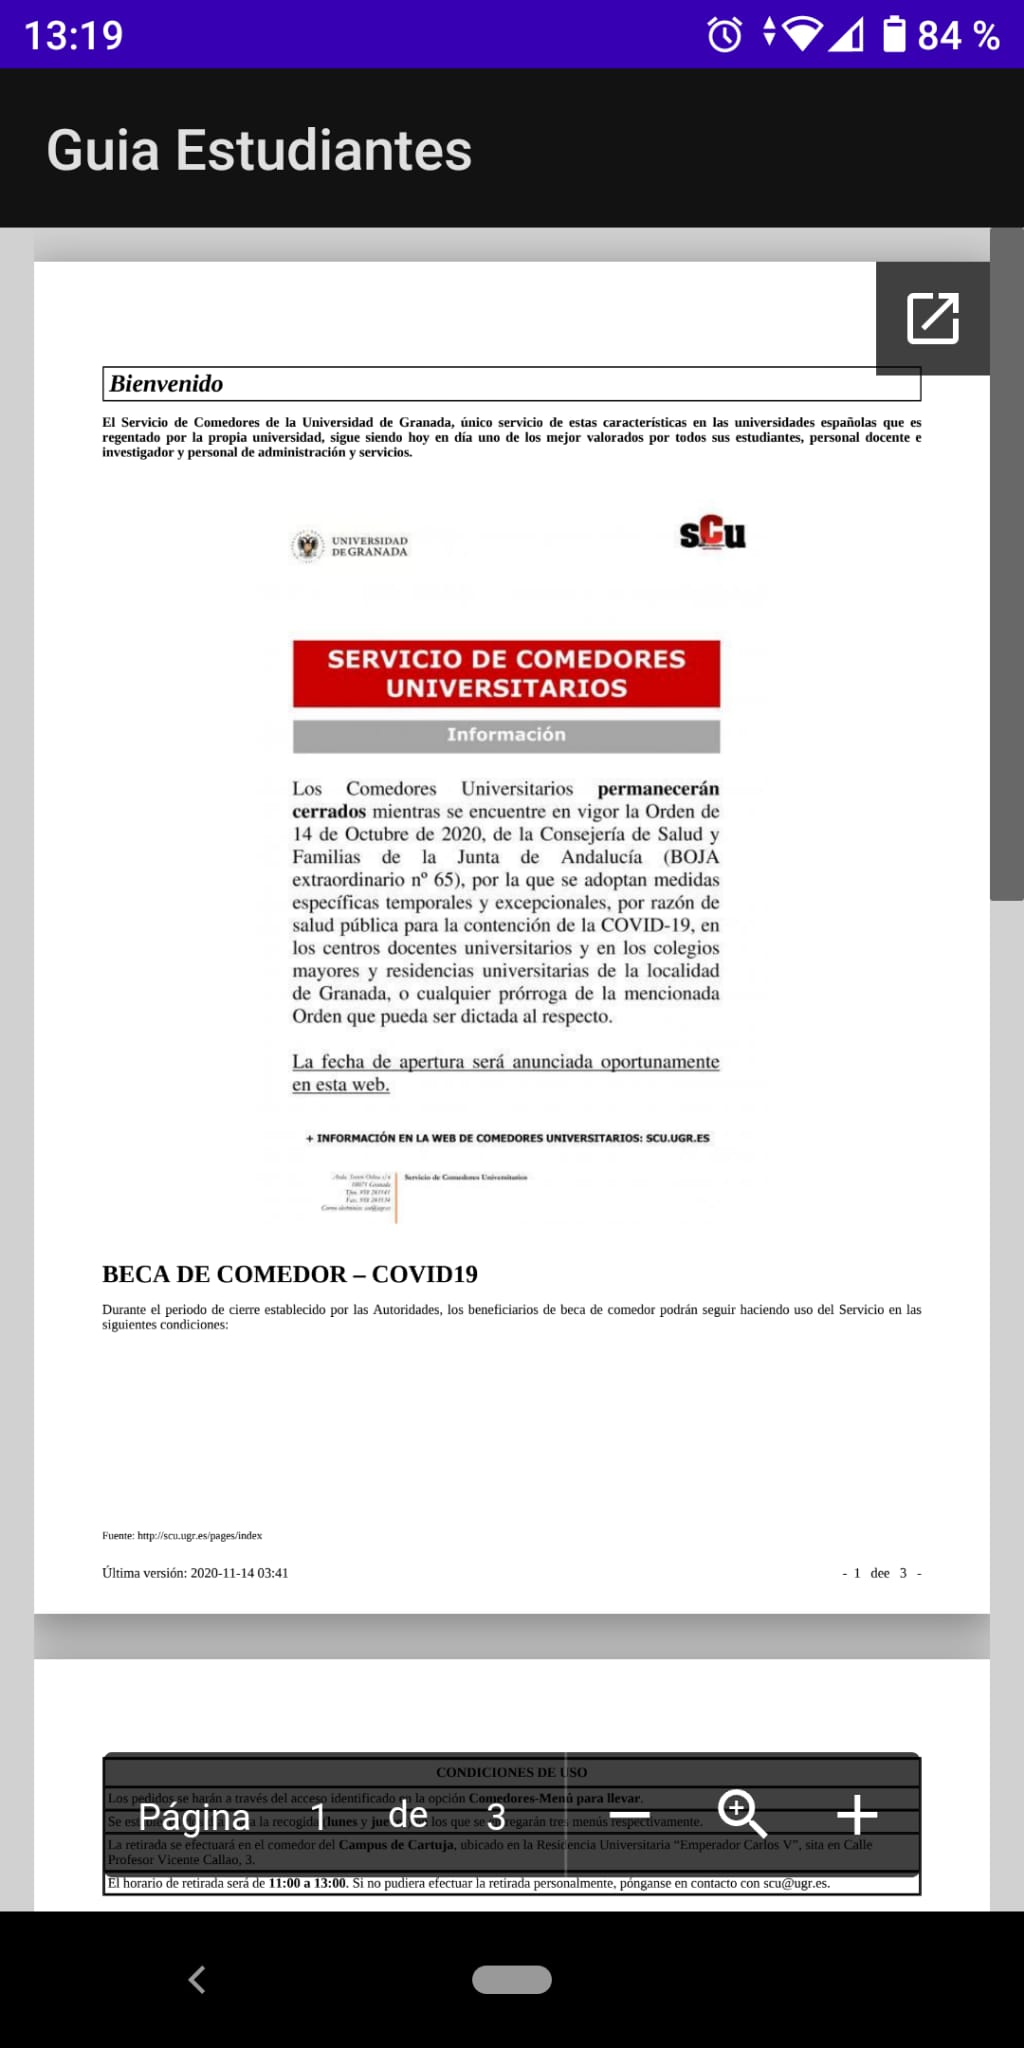
\includegraphics[width=1\linewidth]{comedores.jpeg}
    \caption{PDF comedores cargado}
    \label{fig:sub-second}
  \end{subfigure}
\end{figure}

